
\chapter{Relationen und Graphen}



% Dies wird klar, wenn man bedenkt, dass praktisch jede mathematische Definition von der Form
%\begin{quote}
%``Ein [hier hübscher Name einfügen] ist eine \textbf{Menge} mit folgenden Eigenschaften: [hier interessante Eigenschaften einfügen]''.
%\end{quote}
%ist. In der Mathematik gilt demnach: ``Alles ist Menge''. Alleine diese Feststellung sollte eine genauere Untersuchung des Mengenbegriffes hinreichend motivieren.
%
%Grundsätzlich geht es in der Mengenlehre darum, wie man verschiedene mathematische Objekte zu einem neuen mathematischen Objekt zusammenfassen kann. Also wie man Dinge zusammen
%
%

\section*{Relevanz für die Informatik}
Beziehungen werden in der Mathematik mit Relationen modelliert. Als Modell für ein derart fundamentales Konzept sind Relationen sowohl in der Mathematik als auch in der Informatik nahezu allgegenwärtig. Einige Beispiele von Relationen in der Informatik:
\begin{itemize}
\item Relationale Datenbanken
\item E-R-Diagramme
\item Zustandsklassen von endlichen Automaten
\item Input-Output Relation
\item Funktionen
\item $\vdots$
\end{itemize}
Graphen und (binäre) Relationen sind im wesentlichen gleichwertig, in der Tat können
Graphen auf natürliche Art und Weise dazu verwendet werden, Relationen grafisch
darzustellen. In der Informatik sind Graphen (insbesondere Bäume) eine der
fundamentalen Datenstrukturen (eine Art Daten zu organisieren).


\section*{Lernziele}
Sie kennen
\begin{itemize}
\item den Funktionsbegriff.
\item Äquivalenzrelationen und Äquivalenzklassen sowie ihre grundlegenden Eigenschaften.
\item Ordnungsrelationen (in den verschiedenen Variationen) und ihre grundlegenden
Eigenschaften.
\item grundlegende Typen von Graphen.
\end{itemize}
Sie verstehen
\begin{itemize}
\item den Zusammenhang von Funktionen, Relationen und Graphen.
\item den Zusammenhang von Äquivalenzrelationen und Partitionen.
\item die Problematik der ``Wohldefiniertheit'' von Funktionen auf Faktormengen.
\item wie man Relationen mit Graphen darstellen kann.
\end{itemize}
Sie sind in der Lage
\begin{itemize}
\item (endliche) Ordnungsrelationen als Hasse Diagramme zu skizzieren.
\item eine Ordnungsrelation aus einem Hasse Diagramm abzulesen.
\end{itemize}


\section*{Literatur und Links}
Ergänzende Literatur:
\begin{itemize}
\item \cite{diskreteStrukturen} Kapitel 4.1 bis 4.3.
\item \cite{pareigis} Kapitel 1.4 und 1.5.
\end{itemize}
Nützliche Links:
\begin{itemize}
\item \url{http://de.wikipedia.org/wiki/Relation_%28Mathematik%29}
\item \url{https://de.wikipedia.org/wiki/Graph_(Graphentheorie)}
\end{itemize}


\section{Grundlagen}

Relationen beschreiben Beziehungen zwischen (mathematischen) Objekten. Es soll die ganze Bandbreite an möglichen Beziehungen modelliert werden können. Folgend, vier völlig verschiedene Relationen.
\begin{bsp}
Die Relationen $R_1,R_2,R_3$ und $T$ sind durch folgende Zuordnungen gegeben:
\begin{itemize}
\item Zwei Geraden stehen in Relation $R_1$ zueinander, wenn sie parallel sind. Dies ist eine (binäre) Relation auf der Menge aller Geraden.
\item Zwei Punkte auf der Erdoberfläche stehen zueinander in Relation $R_2$, wenn der erste Punkt zu Fuss (und ohne weitere Hilfsmittel) vom zweiten Punkt aus erreichbar ist.
\item Eine Person $P$ steht in Relation $R_3$ zu Person $Q$, wenn $P$ in $Q$ verliebt ist.
\item Eine natürliche Zahl $x$ steht in Relation $T$ zu einer natürlichen Zahl $y$, falls $x$ ein Teiler von $y$ ist.
\end{itemize}
\end{bsp}

Wie können wir den Relationsbegriff fassen, damit wir möglichst keinen Einschränkungen unterliegen, wenn wir beliebige (auch beliebig exotische) Beziehungen als Relationen modellieren/auffassen wollen? Wie können wir also die Definition einer Relation möglichst weitläufig fassen?

\begin{df}
Eine $n$-Stellige \textit{Relation} $R$ auf den Mengen $A_1,\dots A_n$ ist eine Menge von $n$-Tupeln aus $A_1\times\dots \times A_n$. Mit anderen Worten, die Relationen auf $A_1,\dots,A_n$ sind genau die Teilmengen
\[
R\subseteq \prod_{i=1}^nA_i.
\]
Ist $R$ eine $n$-stellige Relation und gilt $(x_1,\dots,x_n)\in R$, dann sagen wir, dass die Elemente $x_1,\dots,x_n$ zueinander in Relation $R$ stehen.
Eine $2$-stellige Relation $R\subseteq X\times Y$ heisst auch eine \textit{binäre Relation} auf den Mengen $X$ und $Y$.
\end{df}

\begin{ntt}
Ist $R$ eine binäre Relation und sind $x,y$ Elemente mit $(x,y)\in R$ (d.h. $x$ steht in Relation $R$ zu $y$), dann schreiben wir auch $xRy$.
\end{ntt}

Wir werden uns im Folgenden auf binäre Relationen beschränken.

\begin{bsp}\label{Bsp:Geraden}
Wir betrachten die Relation $R_1$ von Beispiel~\ref{ex:Beispiel1relationen} auf der Menge $\{g,h,p,q,r\}$. Die Geraden $g,h,p,q,r$ sind wie im folgenden Bild gegeben:
\begin{center}
%\begin{framed}
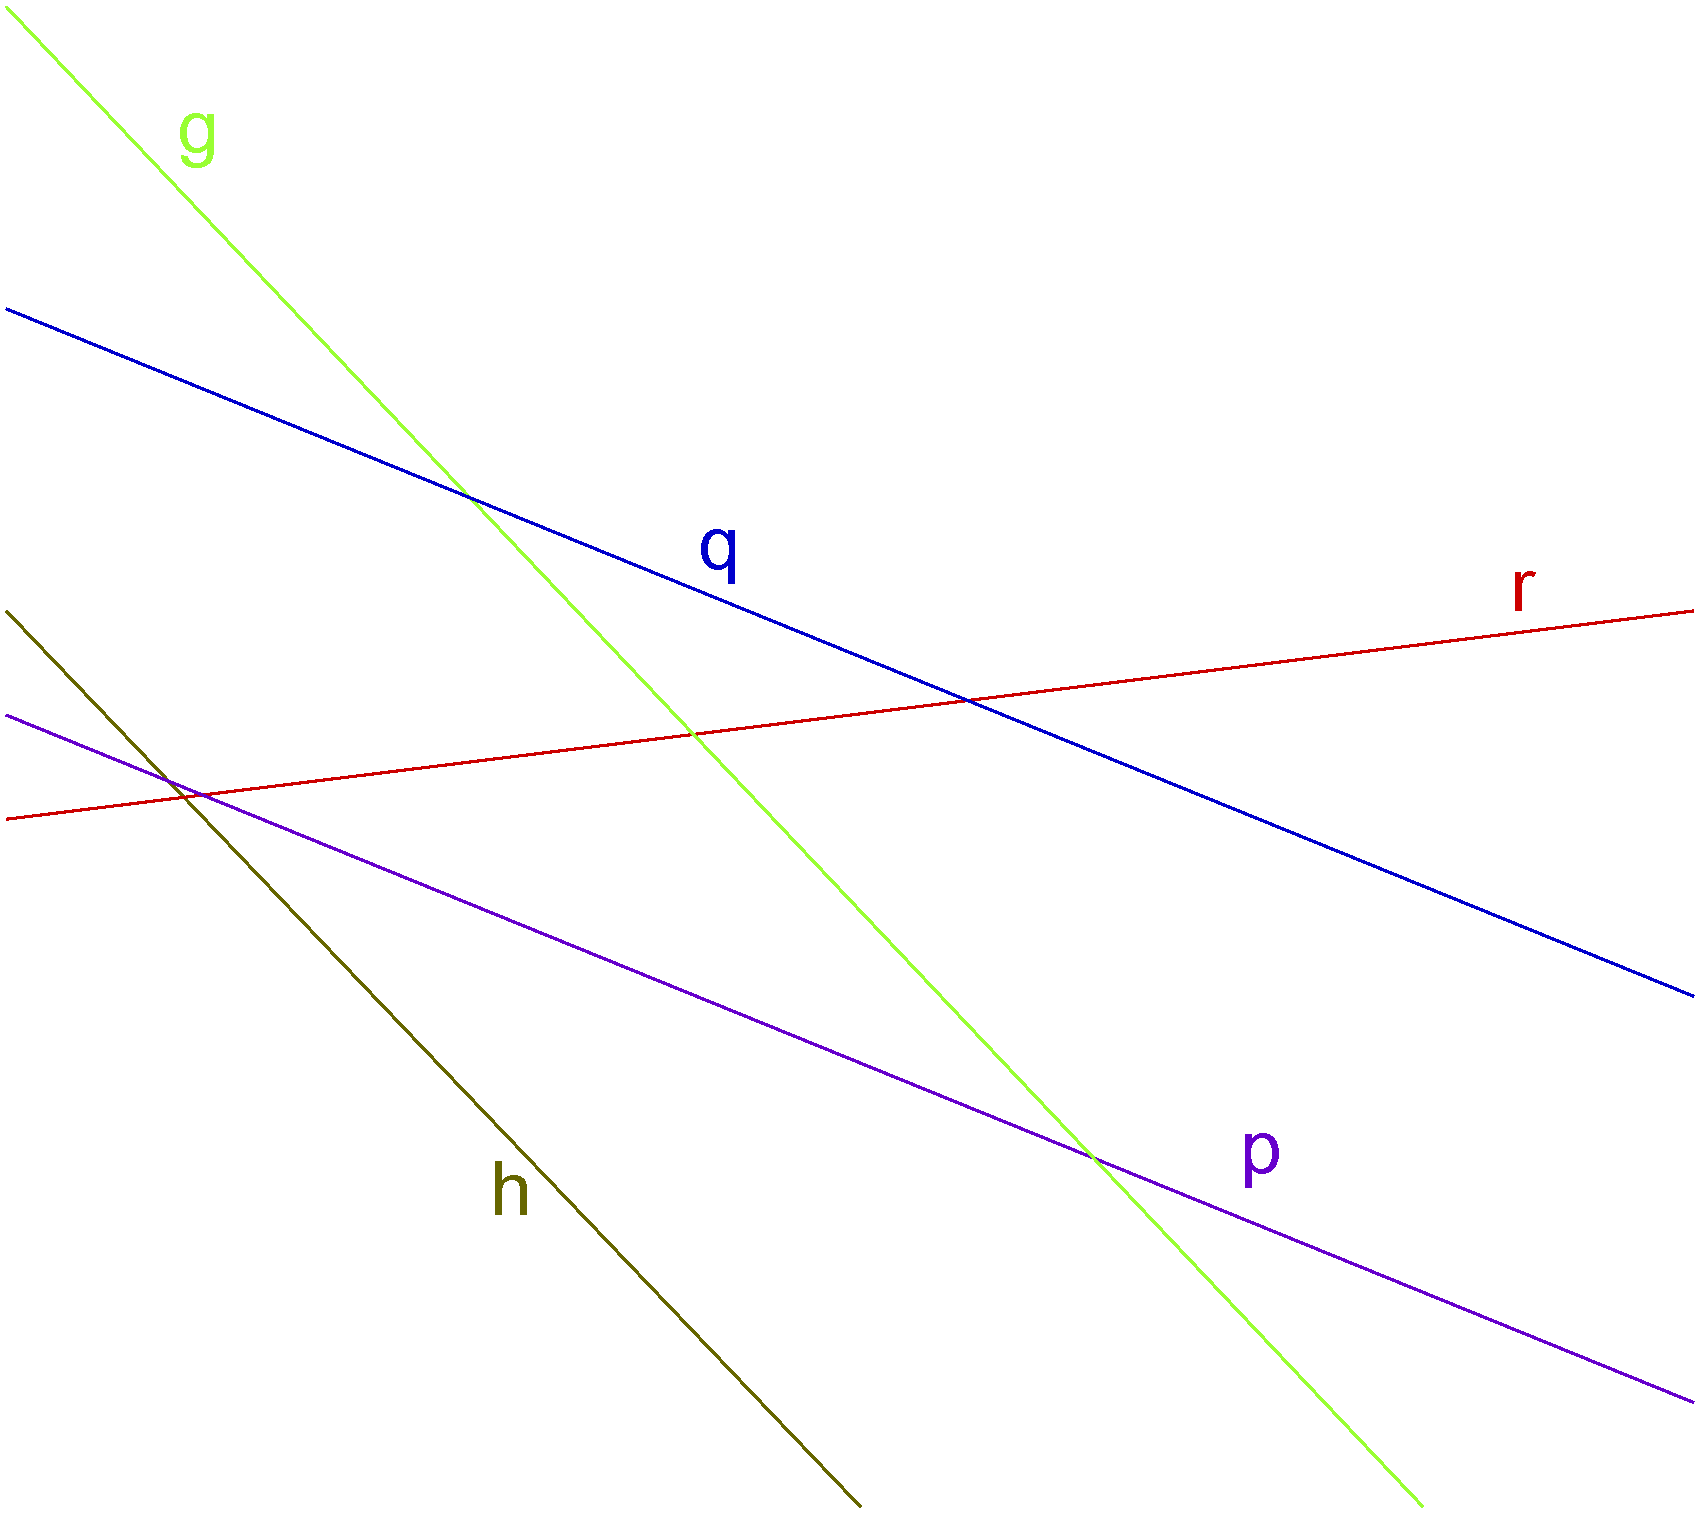
\includegraphics[width=0.5\textwidth]{figures/geraden}
%\end{framed}
\end{center}
Offenbar gelten folgende Beziehungen:
\begin{itemize}
\item Die Gerade $g$ steht in Relation $R_1$ zu folgenden Geraden: $g$, $h$.
\item Die Gerade $h$ steht in Relation $R_1$ zu folgenden Geraden: $g$, $h$.
\item Die Gerade $p$ steht in Relation $R_1$ zu folgenden Geraden: $p$, $q$.
\item Die Gerade $q$ steht in Relation $R_1$ zu folgenden Geraden: $p$, $q$.
\item Die Gerade $r$ steht mit keiner anderen Geraden in Relation $R_1$.
\end{itemize}
Als Menge geschrieben, nimmt die Relation $R_1$ also folgende Gestalt an:
\begin{align*}
R_1=\big\{(g,g),(g,h),(h,h),(h,g),(p,p),(p,q),(q,q),(q,p),(r,r)\big\}.
\end{align*}
Bildlich lässt sich die Relation als Tabelle darstellen:
\begin{center}
\begin{tabular}{ c | c c c c c }
$r$&\xmark&\xmark&\xmark&\xmark&\cmark\\
$q$&\xmark&\xmark&\cmark&\cmark&\xmark\\
$p$&\xmark&\xmark&\cmark&\cmark&\xmark\\
$h$&\cmark&\cmark&\xmark&\xmark&\xmark\\
$g$&\cmark&\cmark&\xmark&\xmark&\xmark\\
\hline
&$g$&$h$&$p$&$q$&$r$
\end{tabular}
\end{center}
Aus der Tabelle erhält man, ähnlich (gleich) wie im Fall von Funktionen und
Funktionsgraphen, den Relationsgraph von $R_1$:
\begin{center}
\begin{tabular}{ c | c c c c c }
$r$&&&&&\cellcolor{black}\\
$q$&&&\cellcolor{black}&\cellcolor{black}&\\
$p$&&&\cellcolor{black}&\cellcolor{black}&\\
$h$&\cellcolor{black}&\cellcolor{black}&&&\\
$g$&\cellcolor{black}&\cellcolor{black}&&&\\
\hline
&$g$&$h$&$p$&$q$&$r$
\end{tabular}
\end{center}
\end{bsp}

\begin{bsp}
Eine schematische Darstellung vom Relationsgraph der Teilbarkeitsrelation (die Relation
$T$ von Beispiel~\ref{ex:Beispiel1relationen}) auf der Menge $\{n\in\N\mid 1<n<100 \}$.
\begin{center}
%\begin{framed}
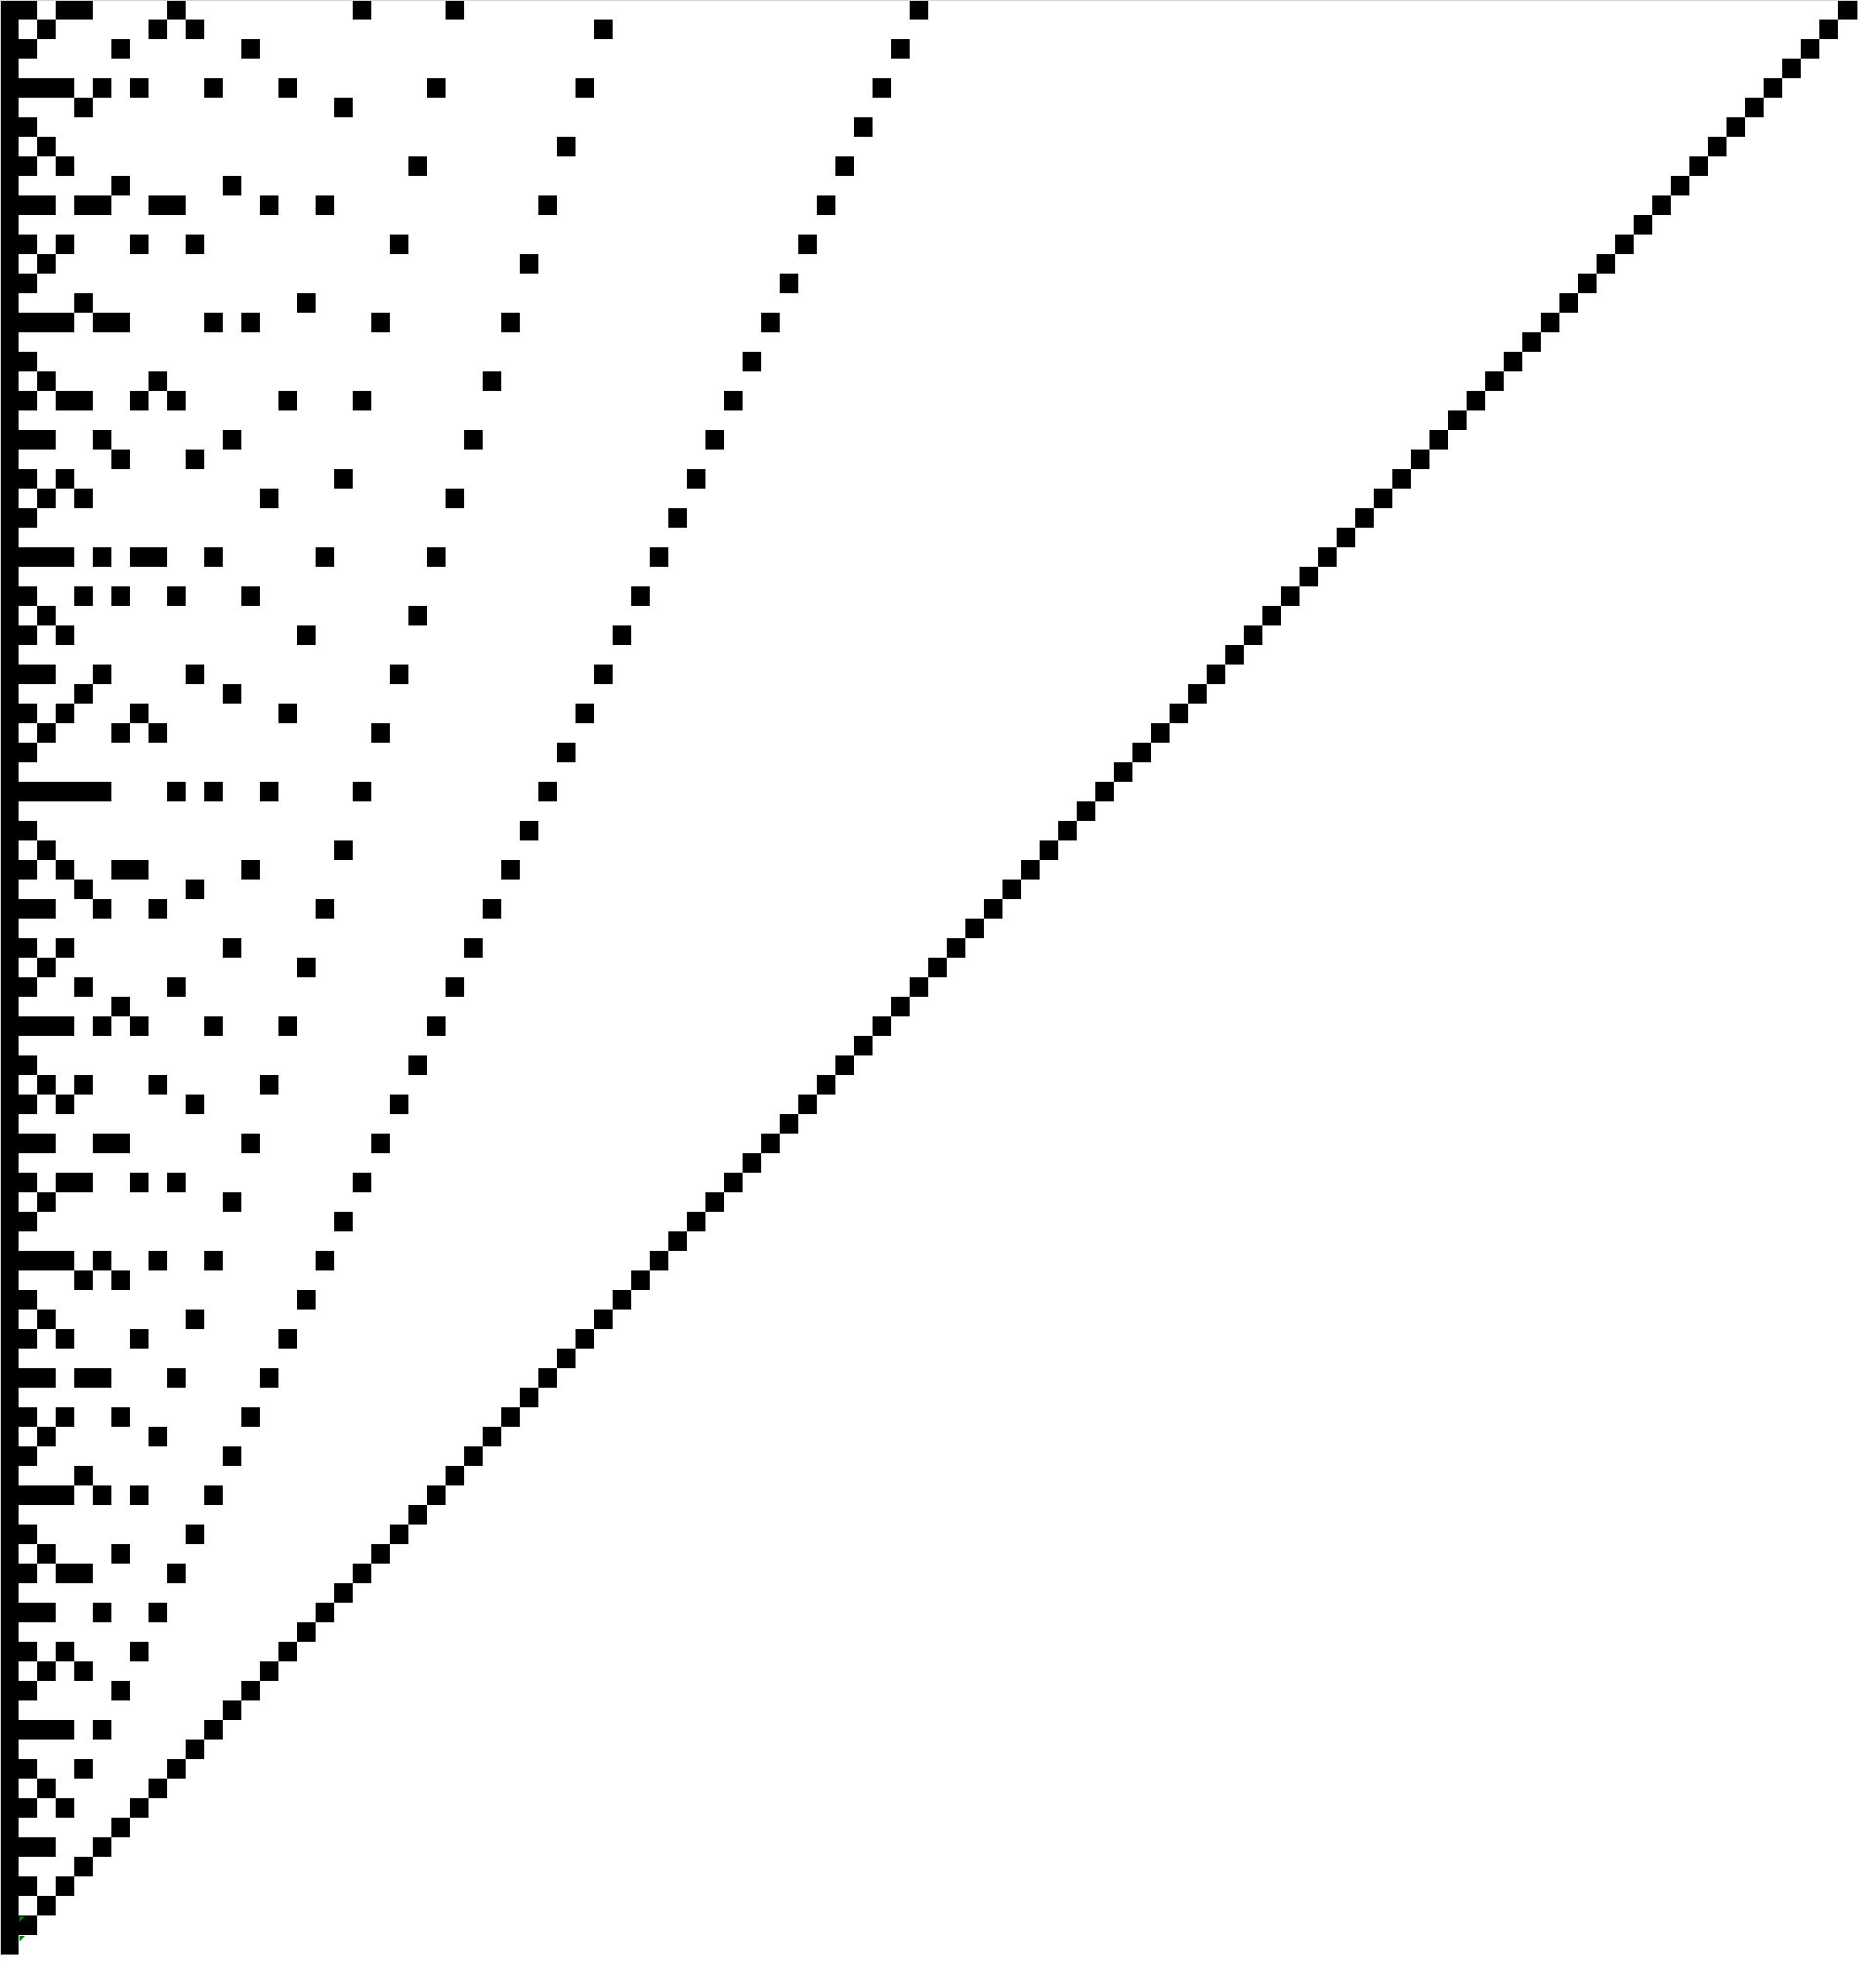
\includegraphics[width=0.2\textwidth]{figures/teiler}
%\end{framed}
\end{center}
Der Relationsgraph von
\[
R=\{(x,y)\mid x,y\in\N\land x,y<100\land x+y\text{ ist ein Vielfaches von }7 \}
\]
\begin{center}
%\begin{framed}

\includegraphics[width=0.2\textwidth]{figures/sum_modulo}
%\end{framed}
\end{center}
\end{bsp}

Ein alternativer Zugang zum Veranschaulichen von binären Relationen bietet die ``Graphentheorie''. Ein Graph\footnote{Nicht zu verwechseln mit einem Funktionsgraphen oder einem
Relationsgraphen} ist in diesem Kontext eine abstrakte Struktur bestehend aus Knoten und Verbindungen zwischen diesen Knoten (Kanten). Endliche Graphen können grafisch dargestellt werden, dazu werden die Knoten durch Punkte und die Kanten durch Linien zeichnerisch repräsentiert.

\begin{df}
    Ein \textit{Graph} ist ein Paar $G=(V,E)$ bestehend aus einer Menge $V$ (Knotenmenge)
    und einer binären Relation $E\subseteq V\times V$ (Kantenmenge).
\end{df}

\begin{bsp}
    Die Teilbarkeitsrelation auf der Menge $\{1,2,3,4\}$ lässt sich als Graph
    $G=(V,E)$ mit
    \begin{align*}
    V &= \{1,2,3,4\}\\
    E &= \{(1,1),(1,2),(1,3),(1,4),(2,2),(2,4),(3,3),(4,4),
    (4,4),(5,5),(6,6)\}
    \end{align*}
    auffassen. Wir veranschaulichen den Graph indem wir die Knoten als Punkte oder Kreise
    und die Kanten als Pfeile zwischen den Knoten darstellen:

    \begin{center}
            \includegraphics[width=0.3\textwidth]{graphviz/g1.png}
    \end{center}


\end{bsp}

\begin{ueb}
    Stellen Sie die Relation $<$ auf der Menge $\{1,2,3,4\}$ als Graph dar.
\end{ueb}
\begin{lsg}~
    \ifthenelse{\boolean{ml}}{
        \begin{center}
            \includegraphics[width=0.3\textwidth]{graphviz/g2.png}
        \end{center}
    }
    {~\answerspace{5cm}}
\end{lsg}

\begin{df}
Eine binäre Relation $R$ auf einer Menge $X$ heisst:
\begin{itemize}
\item \textit{Reflexiv}, wenn für alle $x\in X$
\[
xRx
\]
gilt.
\item \textit{Symmetrisch}, wenn für alle $x,y\in X$
\[
xRy\,\Rightarrow\, yRx
\]
gilt.
\item \textit{Antisymmetrisch}, wenn für alle $x,y\in X$
\[
xRy\land yRx\,\Rightarrow x=y
\]
gilt.
\item \textit{Transitiv}, wenn für alle $x,y,z\in X$
\[
xRy\land yRz\,\Rightarrow \, xRz
\]
gilt.
\end{itemize}
\end{df}


\begin{rk}
Die Relation $R\subseteq X\times X$ ist genau dann reflexiv, wenn die Diagonale
\[
\Delta_X:=\{(x,x)\mid x\in X \}
\]
eine Teilmenge von $R$ ist. Grafisch heisst das, dass die Diagonale (rot markiert) in $R$ enthalten ist.
\begin{center}
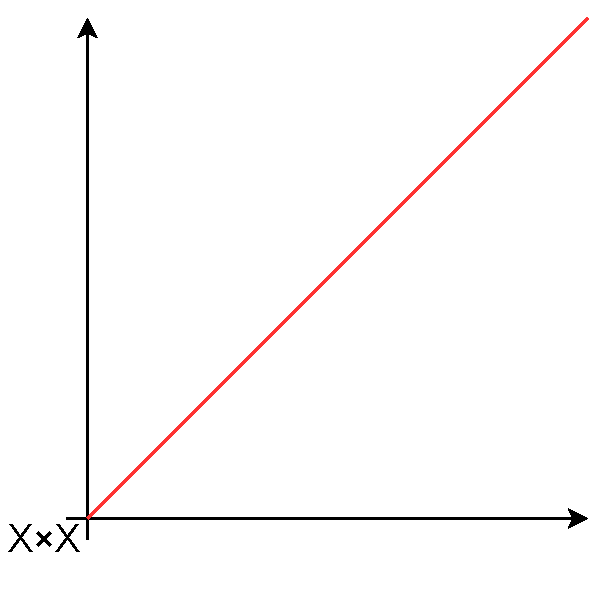
\includegraphics[width=0.2\textwidth]{figures/diagonale}
\end{center}
Die Relation $R$ ist symmetrisch, wenn ihr Graph symmetrisch bezüglich der Geraden $\Delta_X$ ist.
\end{rk}


\begin{bsp}
	Wir betrachten nochmals die Verliebtheitsrelation aus Beispiel \ref{ex:Beispiel1relationen}:
	\[
	pLq:\Leftrightarrow \text{Person $p$ liebt Person $q$.}
	\]
Die Verliebtheitsrelation hat unter anderem folgende Eigenschaften:
\begin{itemize}
	\item $L$ ist nicht reflexiv, da nicht alle Menschen ``selbstverliebt'' sind.
	\item $L$ ist (leider\footnote{Andererseits gäbe es wohl keine Literatur oder gar Kunst, wenn diese Relation tatsächlich symmetrisch wäre.}) nicht symmetrisch, da Liebe nicht immer auf Gegenseitigkeit beruht.
	\item $L$ ist nicht Antisymmetrisch, da es durchaus ``echte'' Liebespaare (aus zwei Partnern bestehend) gibt.
	\item $L$ ist nicht transitiv, da die meisten Leute den angebeteten der eigenen angebeteten nicht lieben (ganz im Gegenteil!).
\end{itemize}
\end{bsp}

\begin{ueb}
	Geben sie binäre Relationen (auf der Menge aller Menschen) mit folgenden Eigenschaften an:
	\begin{enumerate}
		\item Transitiv und nicht antisymmetrisch.
		\item Transitiv, reflexiv und antisymmetrisch.
		\item Nicht reflexiv, nicht transitiv.
	\end{enumerate}
\end{ueb}
\begin{lsg}
	\ifthenelse{\boolean{ml}}{
		Zum Beispiel:
		\begin{enumerate}
			\item $pJq:\Leftrightarrow $ Person $p$ ist jünger als Person $q$.
			\item $pWq:\Leftrightarrow$ Person $p$ hat
			\item $pGq:\Leftrightarrow$ Person $p$ ist vom anderen Geschlecht als Person $q$.
		\end{enumerate}
		}{~
		\answerspace{5cm}
		}
\end{lsg}

\begin{rk}
    Ist $E$ eine symmetrische (binäre) Relation, dann nennt man einen Graph $G=(V,E)$
    \textit{ungerichtet}, andernfalls nennt man $G$ \textit{gerichtet}. Bei gerichteten
    Graphen werden die Verbindungen als Pfeile und bei ungerichteten Graphen als einfache
    Linien dargestellt.
\end{rk}



\section{Äquivalenzrelationen}

Äquivalenzrelationen sind in einem gewissen Sinn (konkret im Sinn von Satz~\ref{satz: equivalenzen verallgemeinerte gleichheit}) verallgemeinerte Gleichheitsrelationen. Sie werden dazu verwendet, (im Sinn der Relation) ähnliche Objekte miteinander zu identifizieren und als ``gleich'' zu behandeln.

\begin{df}
\textit{Äquivalenzrelationen} sind reflexive, symmetrische und transitive Relationen.
\end{df}

\begin{bsp}
Auf jeder Menge $X$ ist die Gleichheitsrelation $\Delta_X=\{(x,x)\mid x\in X \}$ eine Äquivalenzrelation. Weil jede Äquivalenzrelation reflexiv ist, ist die Gleichheitsrelation auf jeder Menge die ``kleinste'' Äquivalenzrelation. Am anderen Ende des Spektrums steht die Relation $X\times X$, sie ist die grösste Äquivalenzrelation auf der Menge $X$.
\end{bsp}

\begin{bsp}
Von den Relationen $R_1,R_2,R_3$ und $T$ aus Beispiel~\ref{ex:Beispiel1relationen}, sind $R_1,R_2$ Äquivalenzrelationen.
\begin{itemize}
\item Die Relation $R_3$ ist keine Äquivalenzrelation, weil sie nicht reflexiv (nicht jeder liebt sich selbst), nicht symmetrisch (es gibt unglücklich Verliebte) und nicht transitiv ist. Man beachte, dass jeder einzelne der genannten Gründe genügt, damit $R_3$ keine Äquivalenzrelation ist.
\item Die Relation $T$ ist zwar reflexiv und transitiv, aber nicht symmetrisch und daher auch keine Äquivalenzrelation.
\end{itemize}
\end{bsp}


\begin{df}
Es sei $R$ eine Äquivalenzrelation auf einer Menge $X$ und $x\in X$. Die \textit{Äquivalenzklasse} $[x]_R$ von $x$ bezüglich $R$ ist die Menge aller Elemente von $X$, die zu $x$ in Relation $R$ stehen:
\[
[x]_R:=\{y\in X\mid xRy \}
\]
Jedes Element einer Äquivalenzklasse nennen wir einen \textit{Repräsentanten} der entsprechenden Äquivalenzklasse. Die \textit{Faktormenge} $\faktor{X}{R}$ \textit{von} $X$ \textit{modulo} $R$ ist die Menge aller Äquivalenzklassen:
\[
\faktor{X}{R}:=\big\{ [x]_R\mid x\in X \big\}
\]
\end{df}

\begin{bsp}\label{bsp:modulo5relation}
Wir betrachten die Relation $\equiv_5$ auf der Menge $\Z$, die wie folgt gegeben ist:
\[
x\equiv_5 y:\Leftrightarrow (x-y)\text{ ist ein Vielfaches von  }5.
\]
Als Java Code könnte man die Relation auch wie folgt darstellen:

\begin{framed}
	\begin{lstlisting}{static,boolean}
static boolean Rel(int x, int y){
    if (y<0) return Rel(x,y+5);
    if (x<0) return Rel(x+5,y);
    if (y>=5) return Rel(x,y-5);
    if (x>=5) return Rel(x-5,y);
    return x == y;
}
\end{lstlisting}
\end{framed}
Wir überzeugen uns nun davon, dass diese Relation eine Äquivalenzrelation ist.
\begin{itemize}
\item \textbf{Reflexivität}: Es gilt für jede ganze Zahl $z$
\[
0\cdot 5=0=(z-z).
\]
Also ist $(z-z)$ ein Vielfaches von $5$, somit gilt $z\equiv_5 z$.
\item\textbf{Symmetrie}: Gilt $x\equiv_5 y$, dann gibt es eine ganze Zahl $z$ mit $5z=(x-y)$. Also ist auch
\[
(y-x)=-(x-y)=-5z=5\cdot(-z)
\]
ein Vielfaches von $5$, d.h. es gilt $y\equiv_5x$.
\item\textbf{Transitivität}: Gilt $x\equiv_5 y$ und $y\equiv_5 z$, dann gibt es ganze Zahlen $r,s$ mit $5r=x-y$ und $5s=y-z$. Insgesamt erhalten wir, dass
\[
x-z=(x-y)+(y-z)=5r+5s=5(r+s)
\]
ein Vielfaches von $5$ ist und somit, dass $x\equiv_5 z$ gilt.
\end{itemize}
Wir betrachten nun die Äquivalenzklassen modulo der Relation $\equiv_5$ (diese heissen Restklassen modulo $5$).
\begin{align*}
[0]_{\equiv_5}&=\{x\in \Z\mid 0\equiv_5y \}\\ &=\{z\in\Z\mid z\text{ ist ein Vielfaches von }5 \}\\
&=\{5z\mid z\in\Z \}\\
\phantom{dd}\\
[1]_{\equiv_5}&=\{x\in \Z\mid 1\equiv_5y \}\\ &=\{z\in\Z\mid \text{ Bei Division durch }5\text{ lässt }z\text{ den Rest }1 \}\\
&=\{5z+1\mid z\in\Z\}\\
\phantom{dd}\\
[2]_{\equiv_5}&=\{x\in \Z\mid 2\equiv_5y \}\\ &=\{z\in\Z\mid \text{ Bei Division durch }5\text{ lässt }z\text{ den Rest }2 \}\\
&=\{5z+2\mid z\in\Z\}\\
\phantom{dd}\\
[3]_{\equiv_5}&=\{x\in \Z\mid 3\equiv_5y \}\\ &=\{z\in\Z\mid \text{ Bei Division durch }5\text{ lässt }z\text{ den Rest }3 \}\\
&=\{5z+3\mid z\in\Z\}\\
\phantom{dd}\\
[4]_{\equiv_5}&=\{x\in \Z\mid 4\equiv_5y \}\\ &=\{z\in\Z\mid \text{ Bei Division durch }5\text{ lässt }z\text{ den Rest }4 \}\\
&=\{5z+4\mid z\in\Z\}
\end{align*}
Die Faktormenge der Relation $\equiv_5$ ist also durch
\[
\faktor{\Z}{\equiv_5}=\{ [0]_{\equiv_5},[1]_{\equiv_5},[2]_{\equiv_5},[3]_{\equiv_5},[4]_{\equiv_5} \}
\]
gegeben.
\end{bsp}
\begin{lm}\label{lm:sim gleiche klasse}
Ist $\sim $ eine Äquivalenzrelation auf einer Menge $X$ und gilt $x,y\in X$ mit $x\sim y$, dann gilt $[x]_\sim=[y]_\sim$. Mit anderen Worten, äquivalente Elemente repräsentieren stets dieselbe Äquivalenzklasse.
\end{lm}
\begin{proof}
Seien $X,\sim,x,y$ wie in der Behauptung. Um zu zeigen, dass $[x]_\sim=[y]_\sim$ gilt, genügt es nachzuweisen, dass $x\sim z\Leftrightarrow y\sim z$ für beliebige $z\in X$ gilt. Wir nehmen $x\sim y$ an, dann gilt
\begin{align*}
y\sim z\Rightarrow x\sim y\land y\sim z \stackrel{\text{Transitivität}}{\Longrightarrow} x\sim z
\end{align*}
und
\[
x\sim z\Rightarrow x\sim y\land x\sim z\stackrel{\text{Symmetrie}}{\Longrightarrow} y\sim x\land x\sim z\stackrel{\text{Transitivität}}{\Longrightarrow} y\sim z,
\]
wie gewünscht.
\end{proof}
\begin{cor}\label{cor:alle Elemente Repräsentanten}
Ist $\sim $ eine Äquivalenzrelation auf $X$ und sind $x,y\in X$ mit $x\in[y]_\sim$, dann gilt $[x]_\sim=[y]_\sim$. Mit anderen Worten, jedes Element einer Äquivalenzklasse ist auch ein Repräsentant dieser Äquivalenzklasse.
\end{cor}
\begin{proof}
Es seien $X,\sim,x$ und $y$ wie in der Behauptung. Aus $x\in[y]_\sim$ folgt $y\sim x$. Die Behauptung folgt nun aus Lemma~\ref{lm:sim gleiche klasse}.
\end{proof}

\begin{satz}\label{satz: equivalenzklassen disjunkt}
Ist $\sim $ eine Äquivalenzrelation auf $X$ und sind $x,y\in X$ mit $[x]_\sim\neq[y]_\sim$, dann gilt $[x]_\sim\cap[y]_\sim=\varnothing$.
Mit anderen Worten, verschiedene Äquivalenzklassen sind immer disjunkt.
\end{satz}
\begin{proof}
Es seien $X,\sim,x$ und $y$ wie in der Behauptung. Wir zeigen die Kontraposition, d.h.
\[
[x]_\sim\cap[y]_\sim\neq\varnothing\Rightarrow [x]_\sim=[y]_\sim.
\]
Es gelte also $[x]_\sim\cap[y]_\sim\neq\varnothing$, es gibt daher ein $z\in [x]_\sim\cap[y]_\sim$. Daraus folgt, dass $x\sim z\land y\sim z$ gilt und wegen der Transitivität und der Symmetrie von $\sim$ folgt sofort $x\sim y$. Die Behauptung folgt nun aus Lemma~\ref{lm:sim gleiche klasse}.
\end{proof}


\begin{satz}\label{satz: equivalenzklassen partition}
Ist $\sim$ eine Äquivalenzrelation auf einer Menge $X$, dann ist die Faktormenge $\faktor{X}{\sim}$ eine Partition von $X$.
\end{satz}
\begin{proof}
Es sei $\sim$ eine beliebige Äquivalenzrelation auf einer Menge $X$. Wir müssen folgende Punkte verifizieren:
\begin{enumerate}
\item\label{a} Die Äquivalenzklassen sind alle nichtleer.
\item\label{2} Die Äquivalenzklassen paarweise disjunkt.
\item\label{3} Es gilt
\[
\bigcup_{x\in X}[x]_{\sim}=X.
\]
\end{enumerate}
Der erste Punkt folgt aus der Definition von der Faktormenge (die Äquivalenzklassen sind via ihrer Repräsentanten definiert). Die Tatsache, dass die Äquivalenzklassen paarweise disjunkt sind, ist genau die Aussage von Satz~\ref{satz: equivalenzklassen disjunkt}. Wir brauchen also bloss noch den letzten Punkt zu verifizieren. Dies folgt, da für jedes $z\in X$, wegen der Reflexivität von $\sim$, $z\sim z$ und somit
\[
z\in[z]_\sim\subseteq\bigcup_{x\in X}[x]_\sim
\]
gilt.
\end{proof}

\begin{rk}
	Das Konzept von Äquivalenzklassen (und deren Zusammenhang mit Partitionen) werden Sie in der theoretischen Informatik in Form von sogenannten ``Zustandsklassen'' wiederfinden, diese werden dort gebraucht, um zu zeigen, dass es Sprachen gibt, die nicht mit ``endlichen Zustandsautomaten'' erkannt werden können.
\end{rk}

\begin{ueb}\label{greg}
	Gegeben Sei die Äquivalenzrelation
	\[
		pRq:\Leftrightarrow\text{$p$ hat am gleichen Tag Geburtstag wie $q$.}
	\]
	Kommentieren Sie folgende Aussagen mit ``wahr'', ``falsch'' oder ``unklar'' unter der
	Annahme $Ray\, R\, Greg $:
	\begin{enumerate}
		\item Ray ist älter als Greg oder Greg ist älter als Ray.
		\item Ray und Greg sind gleich alt.
		\item Ray ist verwandt mit Greg.
		\item Der Altersunterschied von Ray und Greg in Jahren ist ganzzahlig.
	\end{enumerate}
\end{ueb}
\begin{lsg}
	\ifthenelse{\boolean{ml}}{
		$d)$ ist wahr, die restlichen Aussagen sind aufgrund der Annahmen nicht entscheidbar.}
		{~
			\answerspace{2cm}}
\end{lsg}

\begin{ueb}
	Wie viele Äquivalenzklassen hat die Relation $R$ von Übung \ref{greg}?
\end{ueb}
\begin{lsg}
	\ifthenelse{\boolean{ml}}{
		$366$ (Auch in Schaltjahren haben an jedem Tag Leute Geburtstag.)}{~
		\answerspace{1cm}}
\end{lsg}

Wir haben in Satz~\ref{satz: equivalenzklassen partition} gesehen, dass jede 	Äquivalenzrelation auf einer Menge eine Partition auf eben dieser Menge induziert. Als Nächstes sehen wir, dass auch die Umkehrung gilt; jede Partition induziert eine Äquivalenzrelation, deren Faktormenge genau der ursprünglichen Partition entspricht. Insgesamt sehen wir, dass eine eins-zu-eins Korrespondenz zwischen allen möglichen Partitionen und allen möglichen Äquivalenzrelationen auf einer gegebenen Menge existiert.

\begin{satz}
Ist $P=\{A_i\mid i\in I\}$ eine Partition von der Menge $X$, dann ist die Relation $\sim$, gegeben durch
\[
x\sim y:\Leftrightarrow \exists i\in I\,(x\in A_i\land y\in A_i),
\]
eine Äquivalenzrelation auf $X$. Zusätzlich gilt
\[
\faktor{X}{\sim}=P.
\]
\end{satz}
\begin{proof}
Zuerst zeigen wir, dass die Relation $\sim$ unter den gegebenen Umständen eine Äquivalenzrelation ist.
\begin{itemize}
\item \textbf{Reflexivität}: Sei $x\in X$  beliebig. Wir müssen zeigen, dass $x\sim x$ gilt. Da $P=\{A_i\mid i\in I\}$ eine Partition von $X$ ist, gibt es ein $i\in I$ mit $x\in A_i$, daraus folgt sofort $x\sim x$.
\item \textbf{Symmetrie}: Es gelte $x\sim y$. Wir müssen $y\sim x$ zeigen. Aus $x\sim y$ folgt, dass es ein $i\in I$ mit $x\in A_i\land y\in A_i$ gibt, dies ist offensichtlich äquivalent zu $y\sim x$.
\item \textbf{Transitivität}: Es gelte $x\sim y\land y\sim z$. Wir müssen $x\sim z$ zeigen. Aus $x\sim y\land y\sim z$ folgt, dass es $i,j\in I$ gibt so, dass $x,y\in A_i$ und $y,z\in A_j$ gilt. Da $P=\{A_i\mid i\in I\}$ eine Partition ist, kann $y $ nicht in zwei verschiedenen Blöcken enthalten sein, es gilt daher $i=j$ und somit $x\sim z$.
\end{itemize}
Dass die Äquivalenzklassen von $\sim$ genau den Blöcken von $P$ entsprechen ist sofort klar, wenn man beachtet, dass zwei Elemente genau dann äquivalent sind, wenn sie im selben Block von $P$ liegen.
\end{proof}

Am Anfang dieses Abschnittes haben wir Äquivalenzrelationen als verallgemeinerte Gleichheitsrelationen beschrieben, dies können wir im folgenden Satz präzisieren.

\begin{satz}\label{satz: equivalenzen verallgemeinerte gleichheit}
Für jede Relation $\sim$ auf einer Menge $X$ sind folgende beiden Aussagen äquivalent.
\begin{enumerate}
\item[1.] Die Relation $\sim$ ist eine Äquivalenzrelation.
\item[2.] Es gibt eine Menge $Y$ und ein Funktion $F:X\to Y$ so, dass für alle $x,y\in X$
\[
x\sim y\Leftrightarrow F(x)=F(y)
\]
gilt.
\end{enumerate}
\end{satz}
\begin{proof}
Wenn $\sim$ eine Äquivalenzrelation auf der Menge $X$ ist, dann erfüllt die Abbildung
\[
F:X\to\mathcal{P}(X)\phantom{abstand}\text{mit} \phantom{abstand} F(x)=[x]_\sim
\]
alle geforderten Eigenschaften. Ist umgekehrt eine Funktion $F:X\to Y$ wie in der Behauptung gegeben, dann gilt für die Relation $\sim$ Folgendes:
\begin{itemize}
\item\textbf{Reflexivität} gilt, da für jedes Element $x\in X$ trivialerweise $F(x)=F(x)$ gilt.
\item \textbf{Symmetrie} folgt, da für beliebige Elemente $x,y\in X$
\[
x\sim y\Rightarrow F(x)=F(y)\Rightarrow F(y)=F(x)\Rightarrow y\sim x
\]
gilt.
\item\textbf{Transitivität} folgt, da für beliebige Elemente $x,y,z\in X$
\[
x\sim y\land y\sim z\Rightarrow F(x)=F(y)\land F(y)=F(z)\Rightarrow F(x)=F(z)\Rightarrow  x\sim z
\]
gilt.
\end{itemize}
\end{proof}



\begin{bsp}
Es sei $\sim_{14}$ die folgendermassen auf der Menge $Fun(\R)=\{F\mid F:\R\to\R\}$ gegebene Relation:
\[
F\sim G:\Leftrightarrow F(14)=G(14).
\]
Wir betrachten die Funktion
\[
Eval_{14}:Fun(\R)\to \R\phantom{abstand}\text{mit}\phantom{abstand}Eval_{14}(F)=F(14).
\]
Offenbar gilt
\[
F\sim_{14}G\Leftrightarrow Eval_{14}(F)=Eval_{14}(G).
\]
Anhand von Satz~\ref{satz: equivalenzen verallgemeinerte gleichheit} sehen wir also sofort, dass es sich bei $\sim_{14}$ um eine Äquivalenzrelation handelt.
\end{bsp}

\begin{rk}[Wohldefiniertheitsproblem]
Wir betrachten die Relation $\simeq$, die wie folgt auf der Menge $\N$ gegeben ist.
\[
n\simeq m\Leftrightarrow n,m\text{ haben die gleichen Primteiler}.
\]
Nun definieren wir eine Funktion
\[
F:\faktor{\N}{\simeq}\to \N\phantom{abstand}F([x]_\simeq):=x+102.
\]
Es soll zum Beispiel $F([7]_\simeq)=109$ gelten. Sehen Sie ein Problem bei unserem Vorgehen? Ist $F([49]_\simeq)=151$? Es gilt doch $7\simeq 49$ und somit auch $[7]_\simeq=[49]_\simeq$. Sollte dann nicht auch $F([7]_\simeq)=F([49]_\simeq)$ gelten? Natürlich schon! Das Problem, das wir hier haben, nennt man ein \textit{Wohldefiniertheitsproblem}. Es entsteht, wenn man Funktionswerte von Äquivalenzklassen mit Bezugnahme auf deren Repräsentanten definiert, ohne sicherzustellen, dass der Funktionswert nicht von der Wahl der Repräsentanten abhängt.

Sind eine Äquivalenzrelation $\sim$ auf einer Menge $X$ und eine Funktion $F:X\to Y$ gegeben, so erhält man nur dann durch die Zuordnung
\[
\tilde F([x]_\sim):=F(x)
\]
eine wohldefinierte Funktion
\[
\tilde F:\faktor{X}{\sim}\to Y,
\]
wenn die Funktion $F$ mit der Relation $\sim$ verträglich ist. Das heisst, wenn
\[
x\sim y\Rightarrow F(x)=F(y)
\]
gilt.
\end{rk}

\begin{bsp}
Ein Beispiel (vgl.~\ref{bsp:modulo5relation}) für eine wohldefinierte Abbildung
\[
F:\faktor{\Z}{\equiv_5}\to\faktor{\Z}{\equiv_5}
\]
erhalten wir z.B. durch die Zuordnung
\[
F([x]_{\equiv_5}):=[2x+3]_{\equiv_5}.
\]
Um zu sehen, dass diese Funktion tatsächlich wohldefiniert ist, betrachten wir:
\begin{align*}
x\equiv_5 y&\Rightarrow (x-y)\text{ ist Vielfaches von } 5\\
&\Rightarrow\exists z\in\Z\,(5z=x-y)\\
&\Rightarrow \exists z\in\Z\,\big((2x+3)-(2y+3)=2x-2y=2(x-y)=5(2z)\big)\\
&\Rightarrow (2x+3)-(2y+3)\text{ ist ein Vielfaches von }5\\
&\Rightarrow [2x+3]_{\equiv_5}=[2y+3]_{\equiv_5}\\
\end{align*}
\end{bsp}


\section{Ordnungsrelationen}

Unter Ordnungsrelationen fasst man alle Arten von Relationen zusammen, mithilfe derer man
Objekte in gewisser Weise vergleichen und mehr oder weniger eindeutig sortieren kann. Das
Standardbeispiel ist die Ordnungsrelationen $\leq$ auf den verschiedenen Zahlenmengen.

\begin{df}\label{df:minimale elemente}
Es sei $R$ eine binäre Relation auf der Menge $M$.
\begin{itemize}
\item Zwei Elemente $x,y\in M$ heissen $R$-\textit{unvergleichbar}, falls weder $xRy$ noch $yRx$ gilt.
\item Ein Element $x\in X$ einer Teilmenge $X\subseteq M$ von $M$ heisst $R$-\textit{minimal in $X$}, falls es kein anderes Element $y\in X$ mit $yRx$ gibt.
\item  Ein Element $x\in X$ einer Teilmenge $X\subseteq M$ von $M$ heisst $R$-\textit{maximal in $X$}, falls es kein anderes Element $y\in X$ mit $xRy$ gibt.
\end{itemize}
Wenn keine Missverständnisse zu befürchten sind, dann schreiben wir anstelle von $R$-minimal, $R$-maximal und $R$-unvergleichbar auch einfach minimal, maximal und unvergleichbar.
\end{df}

\begin{rk}
Es sei $X$ eine Teilmenge von $M$ und $R$ eine binäre Relation auf $M$.
Die $R$-minimalen Elemente von $X$ entsprechen im Graph $G=(M,R)$ genau den Knoten, bei
denen keine Pfeile enden, die ihren Ursprung in $X$ haben. Die maximalen Elemente
entsprechen den Knoten, von denen alle ausgehenden Pfeile aus der Menge $X$
``hinauszeigen''. Zwei Elemente $x,y\in M$ sind $R$-unvergleichlich, wenn es keine
Verbindung zwischen $x$ und $y$ gibt.
\end{rk}

\begin{ueb}
Die Relation $R$ auf der Menge $M=\{a,b,u,v,x,y,z\}$ sei durch den Graph $(M,R)$ wie folgt
gegeben.
\begin{center}
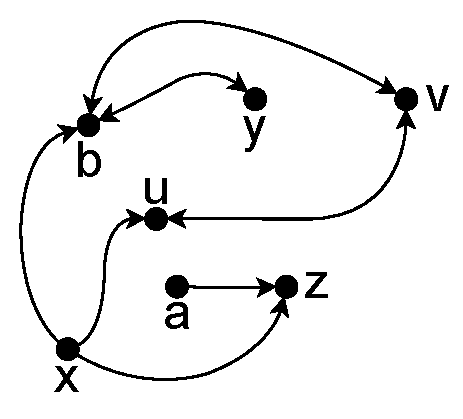
\includegraphics[width=0.5\textwidth]{graphviz/maxmingraph}
\end{center}
Geben Sie alle minimalen und maximalen Elemente von $M$ an.
\end{ueb}
\begin{lsg}~
\ifthenelse{\boolean{ml}}{
	\begin{itemize}
		\item Die minimalen Elemente von $M$ sind $a$ und $x$.
		\item Das einzige maximale Elemente von $M$ ist $z$.
	\end{itemize}
	}{~
	\answerspace{4cm}}
\end{lsg}

\begin{df}
Es sei $R$ eine binäre Relation auf der Menge $M$.
\begin{itemize}
\item $R$ ist eine \textit{Präordnung} auf $M$, wenn $R$ reflexiv und transitiv ist.
\item $R$ ist eine \textit{Halbordnung} auf $M$, wenn $R$ reflexiv, antisymmetrisch und transitiv ist.
\item $R$ ist eine \textit{totale oder lineare Ordnung} auf $M$, wenn $R$ eine Halbordnung ist und keine $R$-unvergleichbaren Elemente existieren.
\item $R$ ist eine \textit{Wohlordnung} auf $M$, wenn $R$ eine totale Ordnung auf $M$ ist so, dass jede Teilmenge $X\neq\varnothing$ von $M$ (mindestens) ein $R$-minimales Element enthält.
\end{itemize}
\end{df}


\begin{bsp}~
\begin{itemize}
\item Die Relation $\leq$ auf der Menge $\R$ ist eine totale Ordnung, die aber keine Wohlordnung ist (die Menge $\{x\in\R\mid 0<x<1\}$ hat kein kleinstes Element). Auf der Menge $\N$ ist $\leq$ eine Wohlordnung\footnote{Ein Beweis dazu kommt im nächsten Kapitel.}. Auf der Menge $\Z$ ist die Relation $\leq$ keine Wohlordnung. Wieso?
\item Ist $A$ eine Menge von Mengen, dann ist die Teilmengenrelation $\subseteq$ eine Halbordnung.
\item Die Teilbarkeitsrelation $T$ auf der Menge $\Z$ ist eine Halbordnung aber keine totale Ordnung. Die Elemente $7$ und $5$ sind $T$-unvergleichlich.
\end{itemize}
\end{bsp}

\begin{df}
    Es sei $R$ eine (binäre) Relation.
    \begin{itemize}
        \item Als \textit{transitiven Abschluss} von $R$ bezeichnet man die kleinste
        (bezüglich $\subseteq$) transitive Relation, die $R$ als Teilmenge enthält,
        sie wird mit $R^+$ notiert.
        \item Die kleinste Relation, die $R^+$ enthält und reflexiv ist, nennt man den
        \textit{reflexiv-transitiven Abschluss} von $R$, sie wird mit $R^*$ bezeichnet.
    \end{itemize}
\end{df}

\begin{rk}
    Für eine beliebige (binäre) Relation $R$ gilt genau dann $xR^*y$, wenn es
    eine endliche Folge $x=k_1,\dots,k_n=y$ gibt, so dass $k_iRk_{i+1}$ für alle
    Indices $i=1,\dots,n-1$ gilt. Es gilt also genau dann $xR^*y$, wenn es eine Folge von
    Elementen gibt, die mit $x$ beginnt, mit $y$ endet und deren Elemente alle der Reihe
    nach in Relation $R$ zueinander stehen. Ist $G=(V,E)$ ein Graph, dann bedeutet
    $xE^*y$, dass in $G$ ein Pfad von $x$ nach $y$ existiert.
\end{rk}

\begin{df}
    Ein \textit{Weg} oder \textit{Pfad} in einem Graph $G=(V,E)$ ist eine endliche Folge
    $k_1,\dots,k_n\in V$ von Knoten, so dass $k_iEk_{i+1}$ für alle Indices
    $i=1,\dots,n-1$ gilt. Die Knoten $k_1$ und $k_n$ bezeichnet man als \textit{Anfangs-}
    und \textit{Endpunkt} des Pfades. Gilt zusätzlich $k_nEk_1$, dann spricht man von
    einem \textit{Zyklus}.
\end{df}


\begin{rk}
    In der Informatik wichtige Datenstrukturen sind sogenannte \textit{DAGs} (von ``directed acyclic graph''), gerichtete zyklenfreie Graphen. Eine der charakteristischen Eigenschaften von DAG's ist die Tatsache, dass sich ihre Elemente auf eine mit der Struktur des Graphen verträgliche Art sortieren lassen. Oft werden Abhängigkeiten von einzelnen Arbeitsschritten eines Prozesses als DAG modelliert, eine mit der Struktur des Graphen verträgliche lineare Ordnung der Knoten entspricht dann einer möglichen Reihenfolge in der die einzelnen Arbeitsschritte abgearbeitet werden können (ohne Abhängigkeiten zu verletzen).
\end{rk}


\begin{df}
    Es sei $M$ eine endliche Menge und $G=(M,E)$ ein DAG. Eine lineare Ordnung $\preceq\subseteq M\times M$ ist eine \textit{topologische Sortierung} von $G$, wenn für alle $a,b\in M$
    \begin{align*}
    a E^* b  \Rightarrow a\preceq b
    \end{align*}
    gilt.
\end{df}

\begin{satz}~
    Jeder endliche DAG besitzt (mindestens) eine topologische Sortierung.
\end{satz}
\begin{proof}
    Wir bemerken zuerst, dass jeder endliche DAG $G=(V,E)$ minimale Elemente bezüglich der Relation $E$ besitzt (wieso?). Weiter bemerken wir, dass jeder DAG, von dem ein minimaler Knoten (zusammen mit den von diesem Knoten ausgehenden Pfeilen) entfernt wird, wieder ein DAG ist (entfernen von Knoten und Verbindungen kann keine neuen Zyklen erzeugen). Aus diesen Beobachtungen folgt, dass folgender Algorithmus eine topologische Sortierung für jeden endlichen DAG generiert:
    \begin{enumerate}
        \item Wenn $G=(V,E)$ nicht leer ist, dann wähle ein bezüglich $E$ minimales Element $x\in V$ (Wenn $V$ leer ist, terminiere).
        \item Wiederhole die erste Instruktion mit $G'=(V\setminus \{x\},\{(a,b)\in E\mid a\neq x \})$ (d.h. erstelle den DAG $G'$ durch Entfernen von $x$ aus $V$ und entfernen von allen von $x$ ausgehenden Kanten in $E$).
    \end{enumerate}
Die Reihenfolge, mit der die Elemente entfernt werden entspricht einer topologischen Sortierung.
\end{proof}


\begin{satz}
    Folgende Aussagen sind äquivalent:
    \begin{enumerate}
        \item $(V,E\setminus \Delta_V)$ ist ein DAG.
        \item $E^*$ ist eine Halbordnung auf $V$.
    \end{enumerate}
\end{satz}
\begin{proof}
    $a)\Rightarrow b)$: Es sei $(V,E)$ ein DAG. Weil $E^*$ nach Definition bereits
    reflexiv und transitiv ist, müssen wir bloss noch zeigen, dass $E^*$
    antisymmetrisch ist. Gilt $xE^*y$, $yE^*x$ und $x\neq y$, dann gibt es
    Pfade $x,a_1,\dots,a_n,y$ und $y,b_1,\dots,b_m,x$ in $(V,E\setminus \Delta_V)$ (eventuell ist das Entfernen von Wiederholungen nötig, vgl. Wandtafel) und daher auch
    einen Zyklus $x,a_1,\dots,a_n,y,b_1,\dots,b_m$. Die Behauptung folgt per
    Kontraposition.

    $b)\Rightarrow a)$: Wenn $E^*$ eine Halbordnung ist, dann existieren aufgrund der
    Antisymmetrie keine Zyklen mit mehr als einem Knoten in $(V,E)$, daher existieren in
    $(V,E\setminus\Delta_V)$ gar keine Zyklen (vgl. Bild Wandtafel).
\end{proof}

\begin{cor}
    Jede endliche Halbordnung kann zu einer linearen Ordnung erweitert werden. Formal, zu jeder Halbordnung $\preceq$ auf einer Menge $M$ gibt es eine lineare Ordnung $\ll$ auf $M$, so dass
    \begin{align*}
    a\preceq b \Rightarrow a\ll b
    \end{align*}
    gilt.
\end{cor}
\begin{proof}
    Wir haben bereits gesehen, dass der Graph $G=(M,\preceq\setminus\Delta_M)$ ein DAG ist. Jede topologische Sortierung von $G$ erfüllt die Behauptung.
\end{proof}

\begin{rk}
Sind zwei Mengen $A$ und $B$ sowie zwei Halbordnungen $<_A$ auf $A$ und $<_B$ auf $B$ gegeben, dann nennt man die Relation
\[
(x,y)\prec (u,v):\Leftrightarrow x<_A u\lor (x=u\land y<_Bv)
\]
die \textit{lexikographische Ordnung} auf $A\times B$. Sind $<_A$ und $<_B$ totale Ordnungen, dann ist auch die lexikographische Ordnung $\prec$ eine totale Ordnung auf $A\times B$.
\end{rk}


\begin{rk}
Wohlordnungen spielen eine wichtige Rolle im Zusammenhang mit rekursiven Strukturen. Die Tatsache, dass eine Wohlordnung keine unendlichen absteigenden Ketten zulässt, stellt sicher, dass Rekursionen entlang dieser Ordnung immer ``terminieren''. Wir werden uns im nächsten Kapitel genauer mit dieser Beziehung auseinandersetzen. Der nächste Satz gibt aber einen ersten Hinweis auf diesen Zusammenhang.
\end{rk}

\begin{satz}
Ist $\preceq$ eine Wohlordnung auf einer Menge $M$, dann gibt es keine unendlich absteigende Folge
\[
a_0\succeq a_1\succeq\dots\succeq a_n\succeq a_{n+1}\succeq\dots
\]
von verschiedenen Elementen aus $M$.
\end{satz}
\begin{proof}
Gibt es eine absteigende Folge $a_0,a_1,\dots$ wie in der Behauptung, dann ist die Menge
\[
\{a_i\mid i\in M\}
\]
eine Teilmenge von $M$, die kein $\preceq$-minimales Element besitzt. Die Relation $\preceq$ kann also in diesem Fall keine Wohlordnung sein. Die Behauptung folgt durch Kontraposition.
\end{proof}

\begin{bsp}
Die im Folgenden definierte Präordnung spielt eine wichtige Rolle in der sogenannten $\mathcal{O}$-Notation zur Beschreibung des Laufzeitverhaltens von Programmen. Die Relation $\leq^*$ ist auf der Menge $\{f\mid f:\N\to\N \}$ wie folgt gegeben:
\[
f\leq^* g:\Leftrightarrow K(g,f)\text{ ist endlich}
\]
wobei
\[
K(g,f)=\{x\in \N\mid g(x)<f(x) \}.
\]
Die Relation $f\leq^* g$ besagt informell, dass die Funktion $f$ nicht schneller als die Funktion $g$ wächst. Die Relation $\leq^*$ ist eine Präordnung aber keine Halbordnung und auch nicht total. Es gibt darüber hinaus unendlich absteigende Folgen von Funktionen bezüglich der Relation $\leq^*$.
\end{bsp}


\begin{ueb}
	Geben Sie zwei $\leq^*$ unvergleichbare Funktionen $f$ und $g$ an.
\end{ueb}
\begin{lsg}
	\ifthenelse{\boolean{ml}}{
		Zum Beispiel
		\begin{align*}
			f(n) =  \begin{cases}
						1&\text{ falls $n$ gerade}\\
						0&\text{ sonst}
					\end{cases}
		\end{align*}
		und
		\begin{align*}
			g(n) =  \begin{cases}
						0&\text{ falls $n$ ungerade}\\
						1&\text{ sonst}
					\end{cases}
		\end{align*}
		}{~
		\answerspace{5cm}}
\end{lsg}

\begin{df}
Es sei $\preceq$ eine Halbordnung auf einer Menge $M$. Das \textit{Hasse-Diagramm} von $R$ ist eine vereinfachte Darstellung des Graphen $(M,\preceq)$.
\begin{itemize}
\item Die Richtung eines Pfeiles $a\to b$ für Elemente $a,b\in M$ wird dadurch zum Ausdruck gebracht, dass sich der Knoten $b$ oberhalb von $a$ befindet.
\item Pfeile zwischen zwei Punkten $a,b$ werden gelöscht, wenn es einen weiteren Punkt $c$ mit $a\preceq c\preceq b$ gibt.
\item Pfeile, die von einem Punkt auf denselben Punkt zeigen (Schleifen), werden weggelassen.
\end{itemize}
\end{df}

\begin{bsp}
Eine Darstellung als Hasse-Diagramm von der Relation $\leq$ auf der Menge $\{1,\dots 5\}$.
\begin{center}
\begin{tikzpicture}[scale=1]
  \node (1) at (0,0) {$1$};
  \node (2) at (0,1) {$2$};
  \node (3) at (0,2) {$3$};
  \node (4) at (0,3) {$4$};
  \node (5) at (0,4) {$5$};
  \draw (1) -- (2) -- (3) -- (4) -- (5);
\end{tikzpicture}
\end{center}
\end{bsp}

\begin{bsp}
Eine Darstellung der Teilbarkeitsrelation auf der Menge Teilermenge von $28$ ($\{1,2,4,7,14, 28 \}$).
\begin{center}
\begin{tikzpicture}[scale=1]
  \node (28) at (1,3) {$28$};
  \node (4) at (0,2) {$4$};
  \node (14) at (2,2) {$14$};
  \node (2) at (1,1) {$2$};
  \node (7) at (3,1) {$7$};
  \node (1) at (2,0) {$1$};
  \draw (1) -- (2) -- (4) -- (28) -- (14) -- (7) -- (1);
  \draw (2) -- (14);
\end{tikzpicture}
\end{center}
\end{bsp}

\begin{bsp}
Die Teilmengenrelation $\subseteq$ auf der Menge $\mathcal{P}(\{a,b,c\})$, als Hasse-Diagramm dargestellt.
\begin{center}
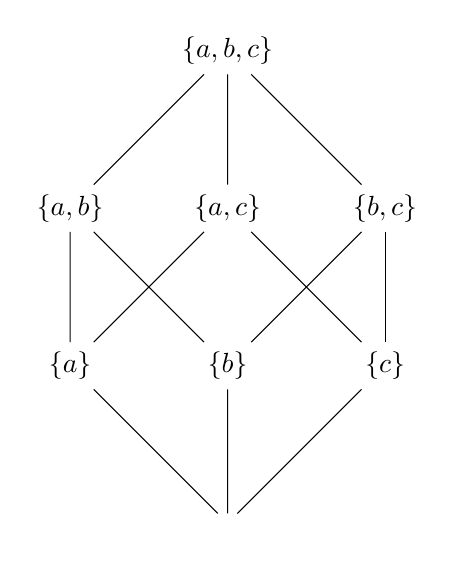
\begin{tikzpicture}[scale=2]
  \node (0) at (1,0) {$\varnothing$};
  \node (a) at (0,1) {$\{a\}$};
  \node (b) at (1,1) {$\{b\}$};
  \node (c) at (2,1) {$\{c\}$};
  \node (ab) at (0,2) {$\{a,b\}$};
  \node (ac) at (1,2) {$\{a,c\}$};
  \node (bc) at (2,2) {$\{b,c\}$};
  \node (abc) at (1,3) {$\{a,b,c\}$};
  \draw (0) -- (a) -- (ab) -- (abc) -- (ac) -- (c) -- (0);
  \draw (0) -- (b) -- (bc) -- (abc);
  \draw (a) -- (ac);
  \draw (b) -- (ab);
  \draw (c) -- (bc);
\end{tikzpicture}
\end{center}
\end{bsp}


\begin{ueb}
Das Hasse-Diagramm einer Halbordnung auf der Menge $\{0,\dots,7 \}$ ist wie folgt gegeben.
\begin{center}
\begin{tikzpicture}[scale=1.5]
  \node (0) at (1,0) {$0$};
  \node (1) at (0,0) {$1$};
  \node (2) at (1,1) {$2$};
  \node (3) at (2,1) {$3$};
  \node (4) at (0,2) {$4$};
  \node (5) at (1,2) {$5$};
  \node (6) at (2,2) {$6$};
  \node (7) at (1,3) {$7$};
  \draw (0) -- (2) -- (5) -- (7) -- (6) -- (3);
  \draw (2) -- (4) ;
  \draw (1) -- (2);
\end{tikzpicture}
\end{center}
\begin{enumerate}
\item Geben Sie alle maximalen und alle minimalen Elemente von der Menge $\{0,\dots,7\}$ an.
\item Geben Sie drei paarweise unvergleichbare Elemente an.
\end{enumerate}
\end{ueb}

\begin{lsg}
	\ifthenelse{\boolean{ml}}{
		\begin{itemize}
			\item Minimale Elemente: $ 0,1,3$
			\item Maximale Elemente: $4,7$
			\item Drei paarweise unvergleichbare Elemente: Z.B. $1,0,3$ oder $4,5,6$ usw.
		\end{itemize}
		}{~
		\answerspace{6cm}}
\end{lsg}


\begin{ueb}
Der Graph $G=(\{12,13,14,18,112 \},\preceq)$ ist wie folgt gegeben.
\begin{center}
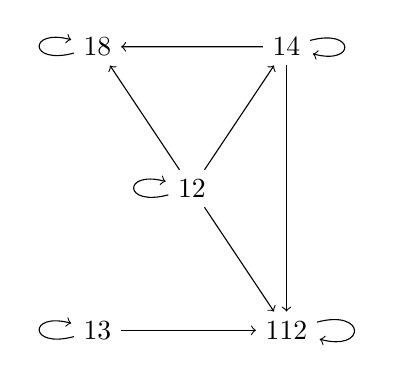
\begin{tikzpicture}[scale=1.2]
  \node (2) at (0,1.5) {$12$};
  \node (3) at (-1,0) {$13$};
  \node (4) at (1,3) {$14$};
  \node (8) at (-1,3) {$18$};
  \node (12) at (1,0) {$112$};
  \path[->] (2) edge (4) edge (8) edge (12) edge [loop left] (2);
  \path[->] (3) edge (12) edge [loop left] (3);
  \path[->] (4) edge (12) edge (8) edge [loop right] (4);
  \path[->] (8) edge [loop left] (8);
  \path[->] (12) edge [loop right] (12);
\end{tikzpicture}
\end{center}
\begin{enumerate}
\item Zeichnen Sie ein Hasse-Diagramm für die Halbordnung $\preceq$.
\item Geben Sie die Relation als Menge an.
\end{enumerate}
\end{ueb}
\begin{lsg}
	\ifthenelse{\boolean{ml}}{
		\begin{enumerate}~
			\item~
				\begin{center}
					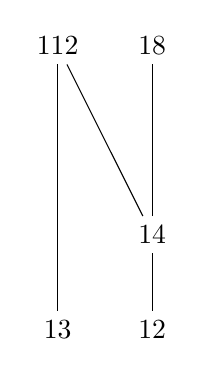
\begin{tikzpicture}[scale=1.2]
					\node (2) at (0,0) {$12$};
					\node (3) at (-1,0) {$13$};
					\node (4) at (0,1) {$14$};
					\node (8) at (0,3) {$18$};
					\node (12) at (-1,3) {$112$};
					\path[-] (2) edge (4);
					\path[-] (3) edge (12);
					\path[-] (4) edge (8);
					\path[-] (4) edge (12);
					\end{tikzpicture}
				\end{center}
			\item $\{(13,13),(13,112),(12,12),(12,112),(12,14),(12,18),(14,14),(14,112),$ $(14,18),(18,18),(112,112) \}$
		\end{enumerate}
		}{~
		\answerspace{6cm}}
\end{lsg}

